% ===========================================================================
% Introducción
% ===========================================================================

\chapter{Introducción}
\label{ch:introduccion}

El Internet de las Cosas (\textit{Internet of Things}, IoT) ha revolucionado la vida cotidiana al permitir el intercambio de datos sin interrupciones entre varios dispositivos a través de Internet. Sin embargo, ha traído consigo desafíos significativos para las aplicaciones que requieren una temporización sincronizada, como garantizar la secuencia ordenada de los datos o el rendimiento sincronizado de las actividades. Las redes de IoT suelen estar compuestas por entidades con recursos variables, lo que dificulta la implementación de métodos de sincronización de tiempo tradicionales en dispositivos con recursos limitados. Las aplicaciones de IoT cubren una amplia gama de necesidades humanas y vitales, desde entornos inteligentes (ciudades, hogar, transporte, etc.) hasta la salud y la calidad de vida~\cite{ayoub2019}.

En este ámbito, las redes inalámbricas de sensores (\textit{Wireless Sensors Network}, WSN) han adquirido un papel importante en una amplia gama de aplicaciones, atribuidas principalmente a su rentabilidad, capacidades funcionales, adaptabilidad y amplia cobertura. Sin embargo, la eficacia de las WSN se ve comprometida por obstrucciones que perjudican la intensidad de la señal y afectan el sincronismo. En consecuencia, la sincronización de reloj es esencial para el funcionamiento de las aplicaciones en redes inalámbricas de sensores, ya que logra mediciones confiables, facilita la coordinación de acciones y garantiza un intercambio de datos fluido entre dispositivos~\cite{yang2020,masalskyi2024}. Las WSN son utilizadas en muchas aplicaciones en las que se requiere una sincronización parcial o completa en la red, como el control de fusión nuclear, la automatización de plantas de fabricación, la comunicación móvil, el diagnóstico de fallos mecánicos, la robótica, el Big Data, el diagnóstico médico y la educación~\cite{balakrishnan2023,lasassmeh2010}.

Los sistemas de control industriales en la era de la Industria 4.0 presentan desafíos significativos desde el punto de vista de la comunicación: baja latencia, confiabilidad y sincronización precisa. En este sentido, las redes sensibles al tiempo (\textit{Time Sensitive Network}, TSN) se han convertido en la principal solución de estos desafíos; por tanto, un requisito estratégico de la sincronización para TSN inalámbricas es lograr que la solución sea autónoma, es decir, que las funcionalidades sean realizadas por la propia red, sin depender de una infraestructura externa~\cite{seijo2022}. Las TSN se basan en cuatro conceptos claves: sincronización de tiempo precisa, baja latencia garantizada, ultra confiabilidad y gestión de recursos. La tecnología inalámbrica ha aportado nuevas posibilidades a las comunicaciones de red, pero los enlaces inalámbricos introducen falta de fiabilidad, canales y latencias asimétricas, interferencia de canal y distorsión de la señal, lo que dificulta el desarrollo de normas e implementaciones adecuadas para el sincronismo en redes inalámbricas~\cite{mildner2019}.

La sincronización de reloj es uno de los temas de investigación más populares en los sistemas distribuidos de medición y control, ya que en estas redes hay un gran número de nodos controlados por relojes independientes y se requiere que cada nodo tenga una referencia de tiempo común~\cite{zhang2024}. Una de las limitaciones más acuciantes es la presencia de retardos asimétricos en los canales de comunicación, ya que son una de las principales razones de la inexactitud del proceso de sincronismo. La presencia de asimetrías puede degradar significativamente el rendimiento de los esquemas de estimación del desfasaje y la desviación del reloj, y desafortunadamente no pueden ser medidas en un sistema de sincronización por pares ni siquiera intercambiando un número infinito de mensajes~\cite{freris2011}. Los protocolos de sincronismo tradicionales asumen que los retardos son simétricos; cuando surge una asimetría en el enlace, estos protocolos crean un desfasaje de reloj significativo. Debido a esta limitación fundamental, los protocolos convencionales no pueden mitigar el desfasaje creado por una asimetría desconocida~\cite{exel2014,oliva2024}.

Dentro de los protocolos existentes, el Protocolo de Tiempo de Precisión Generalizado (\textit{Generalized Precision Time Protocol}, gPTP), definido en IEEE 802.1AS~\cite{ieee8021as_2020}, destaca por ser uno de los pocos especificados para su uso en redes inalámbricas, además de obtener una eficiencia en sincronización en el orden de los nanosegundos. Sin embargo, asume que el retardo de la red es simétrico; por tanto, ante la presencia de asimetrías se ve afectada su eficiencia, lo que puede provocar errores de sincronismo significativos.

En correspondencia con lo expuesto, se propone el siguiente \textbf{problema de investigación}: ¿Cómo mejorar el sincronismo en redes inalámbricas ante la presencia de retardos de propagación asimétricos empleando el protocolo gPTP? A partir de esta problemática se define como \textbf{objetivo general}: Mitigar el efecto de los retardos asimétricos en el sincronismo en redes inalámbricas empleando una versión mejorada del protocolo gPTP. Para dar cumplimiento al objetivo general se plantean los \textbf{objetivos específicos} siguientes:

\begin{enumerate}
\item Realizar una revisión de las bases teóricas relacionadas con el sincronismo en redes inalámbricas, a partir del estudio de la literatura.
\item Analizar las herramientas empleadas y los métodos existentes ---incluyendo técnicas novedosas basadas en filtrado de Kalman--- para mejorar el sincronismo en redes inalámbricas empleando el protocolo gPTP.
\item Implementar una versión mejorada del protocolo gPTP que incorpore un Filtro de Kalman Adaptativo como segunda etapa de corrección de asimetrías.
\item Evaluar el rendimiento de la implementación mejorada en comparación con la implementación de referencia y el protocolo estándar, a través de distintas métricas de precisión y estabilidad.
\end{enumerate}

La \textbf{hipótesis} de la investigación se formula de la siguiente manera: si se emplea una versión del protocolo gPTP que combine la corrección determinista de estampas de tiempo con un filtrado estadístico adaptativo, entonces se logra mitigar los efectos negativos de los retardos de propagación asimétricos con una efectividad superior a la alcanzada por el método de corrección determinista por sí solo, lo que resulta en una mejora significativa adicional en la precisión del sincronismo.

En el desarrollo de la investigación se utilizaron los siguientes \textbf{métodos científicos}: analítico-sintético, inductivo-deductivo, estadístico-matemáticos, medición y modelación.

\begin{figure}[htbp]
  \centering
  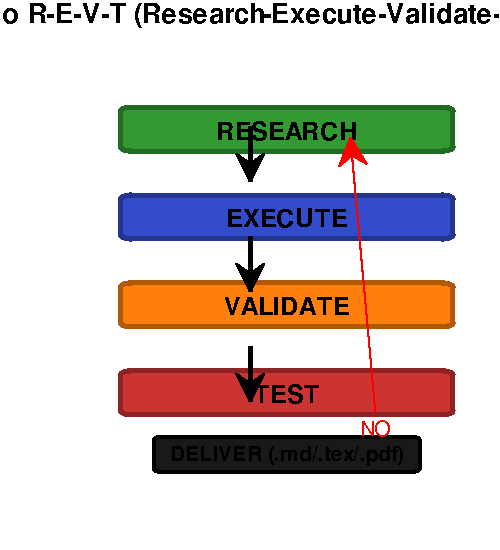
\includegraphics[width=0.55\textwidth]{figures/intro/fig_intro_ciclo_revt}
  \caption{Ciclo iterativo Research-Execute-Validate-Test aplicado en el desarrollo de la investigación.}
  \label{fig:intro_revt}
\end{figure}

\begin{figure}[htbp]
  \centering
  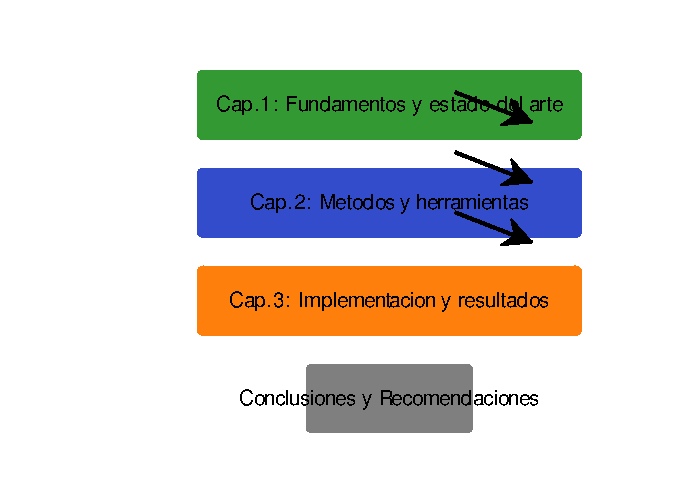
\includegraphics[width=0.6\textwidth]{figures/intro/fig_intro_estructura}
  \caption{Estructura lógica de la tesis.}
  \label{fig:intro_estructura}
\end{figure}

Para su presentación, este trabajo de diploma cuenta con una estructura lógica compuesta por el resumen de la investigación, el índice, la introducción, y tres capítulos donde se desarrolla la investigación. En el \textbf{Capítulo 1} se realiza una revisión bibliográfica que aborda el sincronismo en redes inalámbricas, sus principales aplicaciones en IoT, los desafíos técnicos, el efecto de las asimetrías y una caracterización de los protocolos de sincronización PTP y gPTP. En el \textbf{Capítulo 2} se efectúa un análisis sistemático de 15 métodos existentes para mitigar el efecto de los retardos asimétricos, organizados en siete categorías (corrección determinista, filtros de Kalman, estimación robusta, lógica difusa, aprendizaje computacional, filtros de partículas y programación lineal), y se selecciona y describe en detalle un enfoque híbrido que combina la corrección de Exel con un Filtro de Kalman Adaptativo. El \textbf{Capítulo 3} describe las características de la implementación desarrollada en MATLAB/GNU Octave y presenta los resultados de la simulación Monte Carlo, comparando el rendimiento del método propuesto con el método de referencia Exel y con el protocolo estándar. Finalmente, se expresan las conclusiones y recomendaciones para trabajos futuros, y se incluyen las referencias bibliográficas según la norma IEEE.
